% !TeX spellcheck = en_GB
% !TeX encoding = UTF-8
% !TeX root = ../thesis.tex
\chapter{N-Gram Bug Detection in \scratch{}}\label{chap:methods}
%TODO Unfinished chapter!

\begin{figure}[hbtp]
\centering
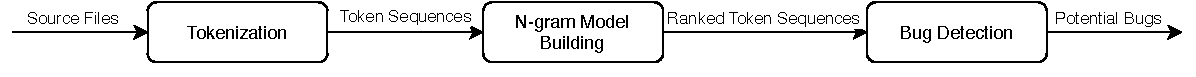
\includegraphics[scale=0.75]{images/Overview.pdf}
\caption{Overview of the n-gram model building process}
\label{fig:overview}
\end{figure}

Figure \ref{fig:overview} visualizes the \ngram{} building process which is explained in this chapter in more detail. In the first section, the tokenization process is described with the way the \scratch{} project is parsed and converted into tokens (Section \ref{sec:tokenization}). The next step is to use the created tokens to build the \ngram{} (Section \ref{sec:model}). Finally, bugs can be detected with the help of the calculated model (Section \ref{sec:detection}).

\section{Tokenization of \scratch{} Code}\label{sec:tokenization}
In order to build a model, we need to tokenize the \scratch{} project into suitable pieces:

\begin{definition}[Token]\label{def:token}
    %
    ``A token is a single fragment of \scratch{} code that is used to partition code into smaller pieces in order to obtain information about its syntax on a specific granularity level.''
    %
\end{definition}

%TODO Rewrite in more detail
It is hard to find the right granularity, but the important thing is that the whole project is represented by the tokens and unusual blocks can be identified. The tokenization process is based on the Abstract Syntax Tree (\AST{}) structure of \litterbox{}. For a simple start, the best way to break the project apart is to identify all drag-and-drop blocks that everyone is familiar with from \scratch{}. After isolating all bigger blocks, the question is how deep to go with the analyzation. I chose to focus on all literals and variables that can be manipulated by the \scratch{} programmer. This approach lead me to excluding all kinds of \AST{}Nodes that were only there for initialization purposes, metadata or even blocks that can only be chosen in a drop-down menu inside a block.  

\section{N-gram Model Building in \scratch{}}\label{sec:model}
%TODO Add introduction to subsections

\subsection{Calculating and Adding N-grams}\label{subsec:n-grams}
Important for the language model is to extract all possible sequences and calculate their probabilities like it is described in Subsection~\ref{subsec:n-grams}. This way a good probability distribution is created that will be the basis for bug detection. For example, given the sequence [GreenFlag, Show, Hide] that is shown in Figure~\ref{fig:sequences}, all its consecutive subsequences are added to the model. In this case the subsequence [GreenFlag, Hide] in Figure~\ref{fig:subsequence} would be the only sequence that is ignored because [Hide] does not immediately follow [GreenFlag]. 

%TODO Fix proportions!
\begin{figure}[t]
    \centering
    \subfigure[A \scratch{} block sequence]{
        \begin{minipage}[t]{0.4\columnwidth}
            \centering
            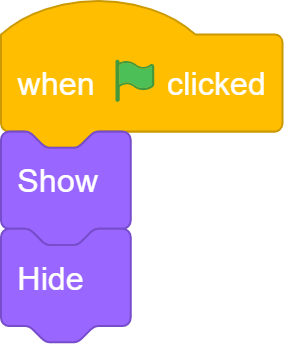
\includegraphics[scale=0.4]{sequence.png}
        \end{minipage}
    }
    \hfill
    \subfigure[Ignored subsequence]{
        \begin{minipage}[t]{0.4\columnwidth}\label{fig:subsequence}
            \centering
            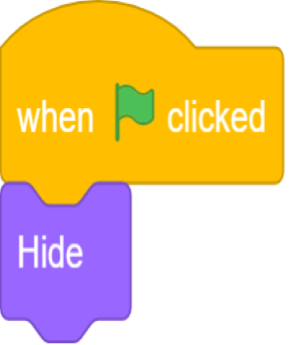
\includegraphics[scale=0.4]{subsequence.png}
        \end{minipage}
    }
    \caption[\scratch{} block sequences]{\label{fig:sequences}\scratch{} block sequences}
    \vspace{-1em}
\end{figure}

%TODO Add example calculation for the probability of the token sequence.

The \hyperref[def:gram_size]{gram size} is an essential part of building a \ngram{}. Existing studies found that 3 to 6-gram models gave the best results, although the optimal \textit{gram size} for bug detection is still unknown. To explore this question more, Section \ref{sec:gram_size} focuses on analysing the effects of different gram sizes in the \scratch{} bug detection as one of the research questions of the bachelor's thesis.

\subsection{Smoothing of Probability Distribution}\label{subsec:smoothing}
If the analysed project is not part of the training dataset, it is important to smooth the probability distribution in order to avoid probabilities of zero. In this implementation, Add-One-Smoothing was utilized which prevents non existent sequences to be shown by adding an additional count to each n-gram. This way there are no sequences with a probability of zero stored in the model. 
%TODO More details about smoothing methods and algorithm with reference


\section{Bug Detection in \scratch{}}\label{sec:detection}
The specific algorithm to find bugs in \scratch{} is implemented the following way. At first, the probabilities of all sequences of the analysed project have to be calculated with help of the model. After that, based on their probability the sequences are ranked and only the ones with the lowest probability get reported as potential bugs. 
%TODO Reference to n-gram probability calculation 

\subsection{Configurations}\label{subsec:configurations}
%TODO Update explanations

\paragraph{Gram Size.}
%TODO Add probability calculation explanation reference
The important point is that a \hyperref[def:markov_chain]{Markov chain} is used to get the conditional probability of a sequence using its n-1 token predecessors as context information. In this work, I built n-gram models with a gram size between 2 to 10 in order to find the optimal n for bug detection in \scratch{} projects (Section \ref{sec:gram_size}. 
\paragraph{Sequence Length.}
The length of analysed sequences of a project is essential to get a detailed analysis of the project structure. The amounts of code blocks and scripts in a \scratch{} project can vary from 1 to a few hundred. By breaking the program into smaller parts, more bugs can be obtained. Finding the right length of a token sequence is evaluated in a more detailed way in Section \ref{sec:sequence_length}.
\paragraph{Reporting Size.}
In contrast to the usual rule-based bug finding techniques which use a probability threshold to distinguish potential bugs from normal sequences, the \ngram{} detects token sequences of low absolute probabilities. The goal is to find the optimal parameter for the reporting size that separates buggy sequences from false positives. A larger amount of bugs that get reported from the found list, will definitely lead to a bigger size of found bugs but also means a higher risk of reporting sequences that are normal occurrences. In this implementation the reporting size is fixed at 25 reports per analysis.
\paragraph{Minimum Token Occurrence.}
Taking out tokens in a project that are not frequently used is a common practice for natural language processing (NLP) techniques. It reduces the chances of falsely reporting uncommon token sequences that are not bugs but just very uncommonly used. However, in this implementation of \ngram{} which is only for \scratch{} analysis purposes the minimum token occurrence is chosen as one. Because of the size difference between usual Java projects compared to normal \scratch{} projects, it would not make sense to filter out any tokens. \scratch{} programmers do not have as much freedom in their implementation because of the restriction through a block-based language and usually choose a different purpose for their programs than text-based programming languages would, which leads to much smaller projects with fewer usages of specific tokens. So, the minimum token occurrence parameter would only make it harder to find low probability sequences in projects which is why I decided not to raise this threshold for my analysis.
\paragraph{Probability Threshold.}
After the analysis of a project a number of sequences with the least calculated probabilities are getting reported as bugs. But in order to minimize the amount of false positives in the bugset, it is common practice to determine a threshold that differentiates a bug from a rare occurrence of a sequence. If a sequence in the report has a probability that is higher than the given threshold, it probably is a normal token sequence that just happens to have a lower probability than the rest of the project's blocks. In this implementation, the threshold is fixed at 0.05.

\subsection{Pruning False Bugs}\label{subsec:false_bugs}
Token sequences with low probability are at the bottom of a n-gram reporting list for potential bugs. But there is always the chance that the found sequence is not actually wrong but just a very unusual or special use case in which its probability would also rank rather low. To find and filter out this kind of false bugs and reduce the candidate bug set, token sequences can only be reported when they are at the bottom of at least two ranked lists of \ngram{s} with the same \textit{gram size} but different \textit{sequence lengths}. This way, sequences are sorted out that just appear on one of these lists and the chance to report false positives gets drastically reduced. 